Como en la sección anterior se ha logrado una implementación correcta de QAOA para un problema simple se continúa con un caso en el que se aplica el algoritmo a un problema distinto, con más qubits y con restricciones.
\\
Estos resultados recopilados corresponden con el problema descrito en la \textit{sección~\ref{sec:4-primer_grafo}}, en el que se resuelve el problema del hallar el camino más corto entre los nodos 0 y 3 para el grafo de la \textit{fig.~\ref{fig:4-primer_grafo}}.

\subsection{Resultados con QAOA}

\subsubsection{Solución del artículo\label{sec:5-primer-paper-resultados-qiskit}}
En las siguientes muestras se ha buscado replicar los resultados del artículo\cite{multi-objective_routing_optimization} del que se ha obtenido el problema.
Para ello se ha tomado el circuito parametrizable incorrecto, mostrado en la \textit{fig.~\ref{fig:4-primer_paper_circuito}}.
La prueba de la igualdad entre la implementación propia y la del artículo se encuentra en que, empleando los parámetros $\beta = 0.28517317$ y $\gamma = -5.05969577$ dados como óptimos, se obtiene un gráfico muy similar al del artículo (\textit{fig~\ref{fig:5-primer-grafo/sin restriccion extra/primer paper aer resultado}}).
El nivel de precisión dado en los parámetros es superior al requerido, ya que con una precisión de 3 o 4 decimales se obtienen los mismos resultados.

\begin{figure}[Resultados QAOA {--} artículo de Urgelles \textit{et al.} (2022) {--} comparación entre resultados]{fig:5-primer-grafo/sin restriccion extra/primer paper aer resultado}{Comparación entre resultado de QAOA obtenido y resultado del artículo\cite{multi-objective_routing_optimization}}
  \subfigure{Resultado del artículo\cite{multi-objective_routing_optimization}}{
    \centering
    \includegraphics[width=0.42\textwidth]{primer-grafo/sin_restriccion_extra/primer_paper_orig_resultado.png}
  } \hfill
  \subfigure{Resultado obtenido}{
    \centering
    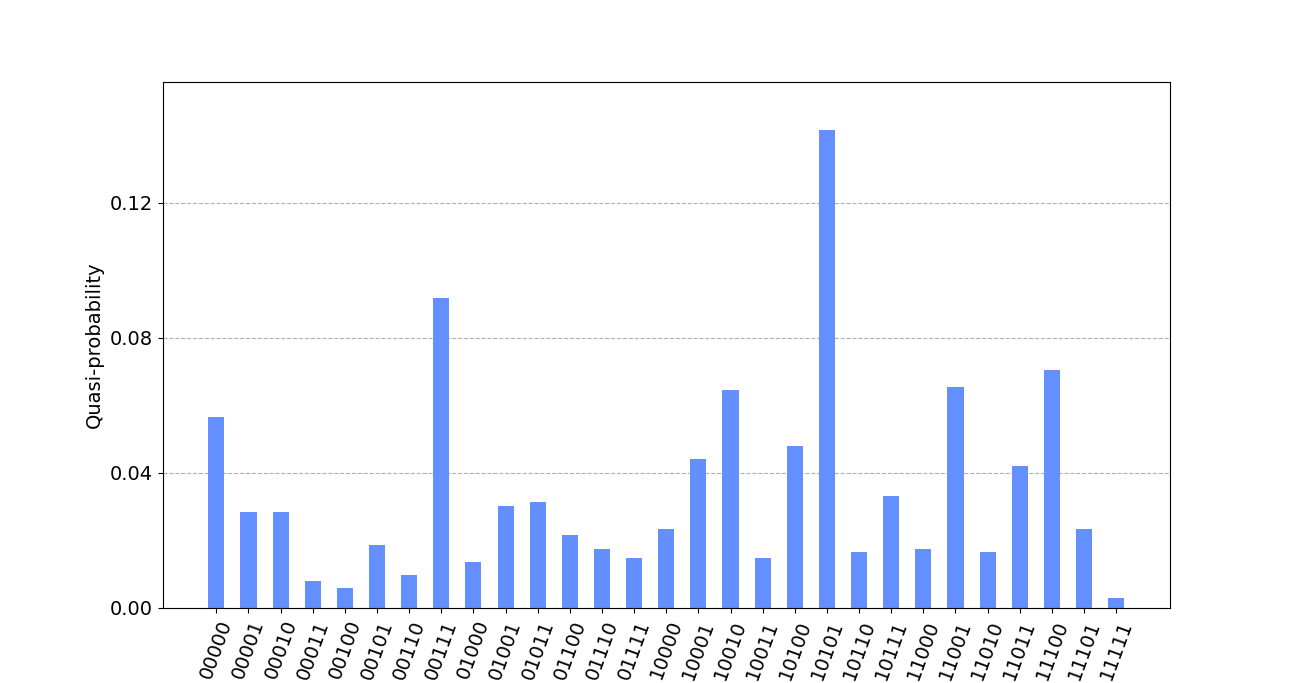
\includegraphics[width=0.49\textwidth]{primer-grafo/sin_restriccion_extra/primer_paper_aer_resultado.png}
  }
\end{figure}

De esta forma, se asume que los resultados del artículo deberían ser equivalentes a los obtenidos en esta instancia del algoritmo.

\begin{table}[Resultados QAOA {--} artículo de Urgelles \textit{et al.} (2022) {--} solución del artículo]{tab:5-primer-paper-aer_estadisticas}{Resultados de la ejecución de la versión de QAOA del artículo\cite{multi-objective_routing_optimization}}
  \centering
  \begin{tabular}{|c|r|r|}
    \hline
    \textbf{nº Capas} & \textbf{NA/TE} & \textbf{MM/TE} \\ \hline
    p = 1 & 91.3\% & 39.34\% \\ \hline
    p = 2 & 64.6\% & 24.16\% \\ \hline
    p = 3 & 63.4\% & 18.82\% \\ \hline
    p = 4 &  9.4\% &  5.38\% \\ \hline
    p = 5 & 67.9\% & 19.45\% \\ \hline
    p = 6 & 29.8\% & 12.59\% \\ \hline
    p = 7 & 28.9\% &  9.12\% \\ \hline
    p = 8 & 36.7\% & 12.49\% \\ \hline
  \end{tabular}
\end{table}

En la \textit{tabla~\ref{tab:5-primer-paper-aer_estadisticas}} se puede observar cómo, en comparación con resultados posteriores de problemas del camino más corto, el caso para $p = 1$ exhibe un comportamiento inusualmente bueno.
Esto contrasta con los resultados con valores de capas más altos para los que, al contrario de lo esperado teóricamente, el rendimiento empeora.

Además, la gran diferencia entre los resultados dados por las estadísticas \textbf{NA/TE} y \textbf{MM/TE} denotan una gran cantidad de ruido al ejecutar el algoritmo, lo cual se corrobora viendo los resultados de ejecuciones concretas, como los dados en la \textit{fig.~\ref{fig:5-primer-grafo/sin restriccion extra/primer paper aer resultado}}.

El resultado de la función gamma es el siguiente:
\begin{figure}[Resultados QAOA {--} artículo de Urgelles \textit{et al.} (2022) {--} función gamma de la solución del artículo]{fig:5-primer_grafo/sin_restriccion_extra/primer_paper_p_27_gamma_fun}{Función gamma de \textit{execute\_circuit()} (con $\beta = 1.0$ y variando $\gamma$). Solución del artículo\cite{multi-objective_routing_optimization}}
  \centering
  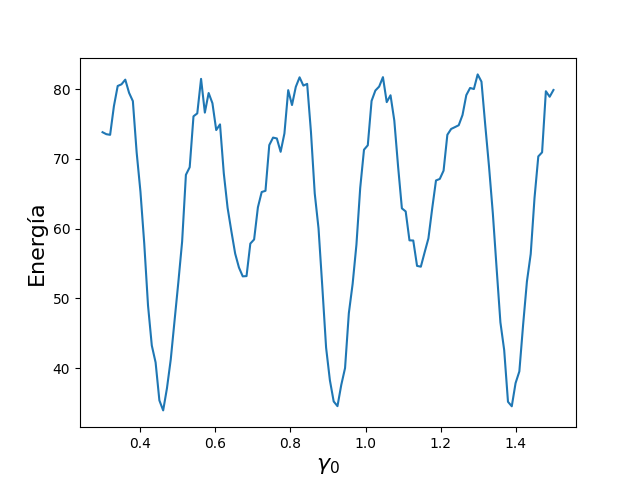
\includegraphics[scale=0.5]{primer-grafo/sin_restriccion_extra/primer_paper_p_27_gamma_fun.png}
\end{figure}

Se puede ver que existen un gran número de mínimos locales, lo cual dificulta la tarea del optimizador clásico.
Haciendo una prueba empleando como parámetros iniciales $(\beta = 1.0, \gamma = 0.5)$, muy cercanos al mínimo, se obtiene el camino óptimo el 100\% de las ejecuciones, lo que sugiere que el problema se encuentra en que el optimizador clásico no encuentra el mínimo de la función \textit{execute\_circuit()}.

Este proceso de inicializar los parámetros con valores concretos no sería una solución válida, ya que se trata de una metodología no automática en la que, para ejecutar correctamente el algoritmo, se necesitaría conocer antes su propio resultado. Además la ejecución correcta sucede para $p = 1$, pero al igual que el caso por defecto $(\beta = 1.0, \gamma = 1.0)$, no escala correctamente al aumentar el número de capas.

\subsubsection{Soluciones según el desarrollo seguido en el trabajo}

Tomando como punto de partida el circuito de la \textit{fig.~\ref{fig:4-primer_circuito}}, correspondiente con el desarrollo correcto de QAOA, se obtienen los siguientes resultados.

Las estadísticas obtenidas en la \textit{tabla~\ref{tab:5-primer-mod_originales-aer_estadisticas}} no dan ningún resultado satisfactorio.
\\
Se aprecia un comportamiento cíclico, similar al que se verá en los resultados del grafo de la \textit{tabla~\ref{tab:5-zhiqiang_mod-orig_estadisticas}}.
La tendencia observada es que se mejoran las estadísticas hasta las 3 capas y luego disminuyen.

\begin{table}[Resultados QAOA {--} artículo de Urgelles \textit{et al.} (2022) {--} implementación de QAOA]{tab:5-primer-mod_originales-aer_estadisticas}{Resultados de la ejecución de QAOA con la solución según el desarrollo del trabajo}
  \centering
  \begin{tabular}{|c|r|r|}
    \hline
    \textbf{nº Capas} & \textbf{NA/TE} & \textbf{MM/TE} \\ \hline
    p = 1 &  0.5\% &  4.05\% \\ \hline
    p = 2 &  9.2\% &  5.83\% \\ \hline
    p = 3 & 54.8\% & 12.98\% \\ \hline
    p = 4 & 11.1\% &  7.00\% \\ \hline
    p = 5 &    6\% &  5.71\% \\ \hline
  \end{tabular}
\end{table}

La función gamma resultante se muestra en la \textit{fig.~\ref{fig:5-primer-mod_originales-gamma_fun}}.
Tiene un mínimo global menos claro con respecto a la función gamma de la versión del circuito del artículo, en la \textit{fig.~\ref{fig:5-primer_grafo/sin_restriccion_extra/primer_paper_p_27_gamma_fun}}.
Además a diferencia de dicha gráfica, en esta no se aprecia periodicidad alguna.

\begin{figure}[Resultados QAOA {--} artículo de Urgelles \textit{et al.} (2022) {--} función gamma de la implementación de QAOA]{fig:5-primer-mod_originales-gamma_fun}{Función gamma de \textit{execute\_circuit()} (con $\beta = 1.0$ y variando $\gamma$). Solución según el desarrollo del trabajo.}
  \centering
  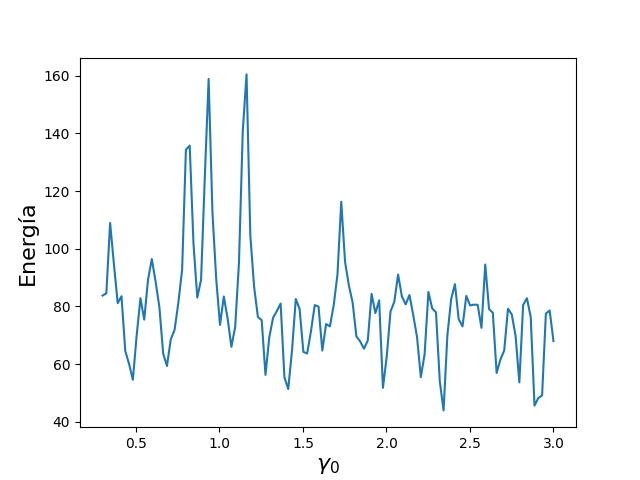
\includegraphics[scale=0.5]{primer-grafo/sin_restriccion_extra/primer-paper-mod_originales-gamma_fun.png}
\end{figure}

Se han realizado modificaciones al algoritmo, mostradas y discutidas en la \textit{sección~\ref{sec:8-primer}} del apéndice.

\subsection{Resultados con QAOA en computador cuántico real}
Utilizando la herramienta \textit{Runtime} de Qiskit se han realizado ejecuciones del código para comprobar sus resultados en computadores reales.

El funcionamiento ha consistido en obtener los parámetros $\gamma$ y $\beta$ en dichos computadores y después ejecutar una vez más en un simulador para obtener el resultado al problema.

\subsubsection{\(p = 1\)}
El código ha sido ejecutado con la imprecisión encontrada en el artículo\cite{multi-objective_routing_optimization} (\textit{sección~\ref{sec:4-primer_grafo_diferencias_con_el_articulo}}), tratando así de asemejarse a los resultados que ahí se exponen.

El resultado obtenido ha sido el siguiente:

\begin{verbatim}
    message: Optimization terminated successfully.
    success: True
     status: 1
        fun: 52.81120901157566
          x: [ 7.624e-01  4.636e-01]
       nfev: 30
      maxcv: 0.0
\end{verbatim}

Este mensaje es devuelto por el optimizador clásico COBYLA y significa que se han encontrado los parámetros $\gamma = 0.7624$ y $\beta = 0.4636$, con los que la función \textit{execute\_circuit()} devuelve un valor de $52.81$.
Esto está muy lejos de ser una media óptima, ya que esta se daría al obtener en todos los casos el camino más corto, lo que daría una media de 11 (el coste de dicho resultado).
El otro valor a remarcar, \textit{nfev=$30$}, se refiere al número de llamadas a la función \textit{execute\_circuit()} realizadas.

Los parámetros obtenidos, ejecutados en un simulador, dan el resultado de la fig.~\ref{fig:5-primer_grafo/sin_restriccion_extra/primer-runtime-mod_paper-1_capa-nairobi_aer}.

\begin{figure}[Resultados QAOA {--} artículo de Urgelles \textit{et al.} (2022) {--} ejecución en simulador]{fig:5-primer_grafo/sin_restriccion_extra/primer-runtime-mod_paper-1_capa-nairobi_aer}{Ejecución de $\gamma, \beta$ en simulador}
  \centering
  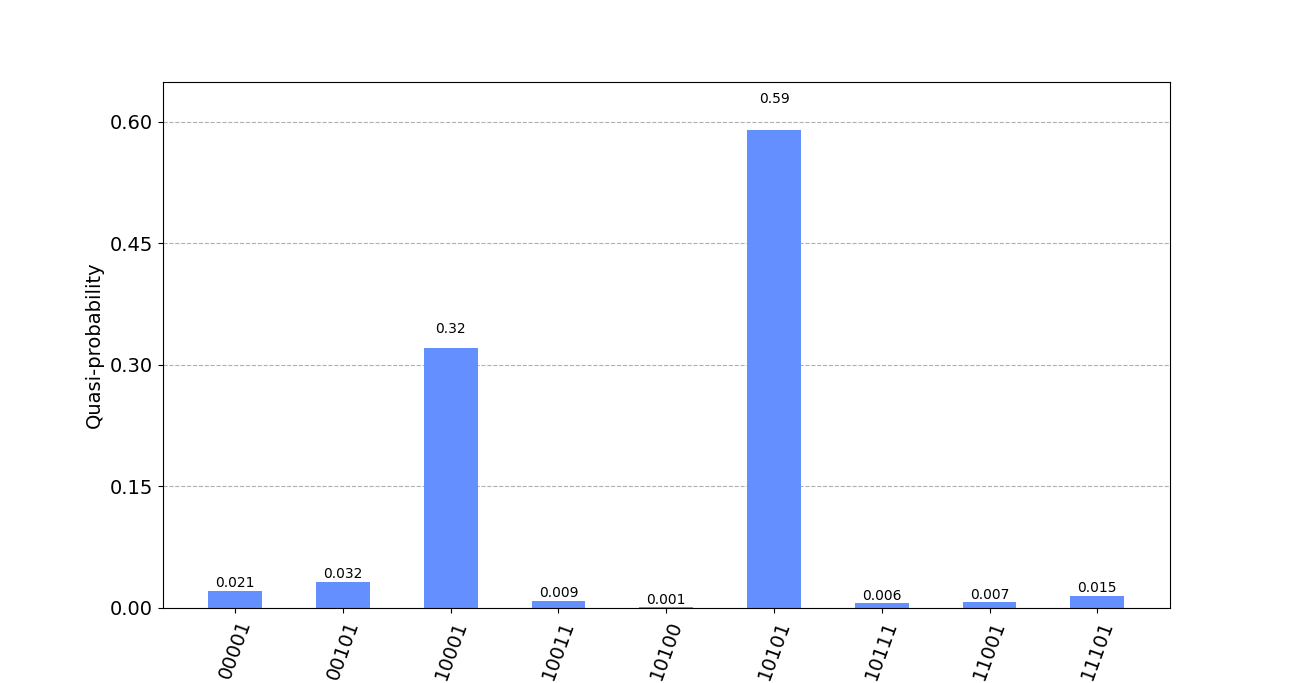
\includegraphics[scale=0.4]{primer-grafo/sin_restriccion_extra/primer-runtime-mod_paper-1_capa-nairobi_aer.png}
\end{figure}

Esto indica que el motivo de obtener un resultado inesperadamente alto de la función se debe a la presencia de un camino, \textit{10001}, de coste elevado obtenido un gran número de veces. Este camino es costoso, con valor de 63, debido a que rompe varias restricciones de la función de coste.

Estos mismos parámetros resultados de la ejecución en \textit{ibm\_nairobi} han sido ejecutados en el computador de \textit{ibm\_lagos}, dando los resultados de la \textit{fig.~\ref{fig:5-primer_grafo/sin_restriccion_extra/primer-runtime-mod_paper-1_capa-nairobi_lagos}}.

\begin{figure}[Resultados QAOA {--} artículo de Urgelles \textit{et al.} (2022) {--} ejecución en computador real]{fig:5-primer_grafo/sin_restriccion_extra/primer-runtime-mod_paper-1_capa-nairobi_lagos}{Ejecución de $\gamma, \beta$ en \textit{ibm\_lagos}}
  \centering
  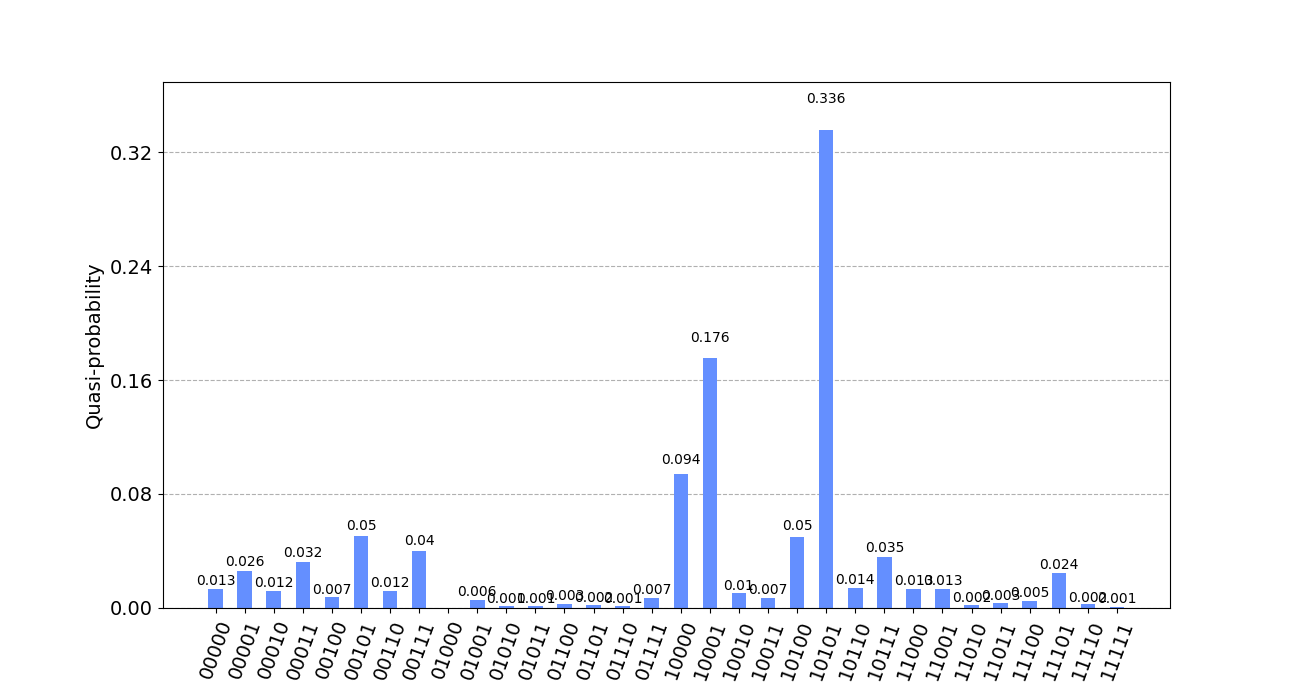
\includegraphics[scale=0.4]{primer-grafo/sin_restriccion_extra/primer-runtime-mod_paper-1_capa-nairobi_lagos.png}
\end{figure}

Comparando las \textit{fig.~\ref{fig:5-primer_grafo/sin_restriccion_extra/primer-runtime-mod_paper-1_capa-nairobi_aer}} y \textit{fig.~\ref{fig:5-primer_grafo/sin_restriccion_extra/primer-runtime-mod_paper-1_capa-nairobi_lagos}}
se aprecia la diferencia de ejecutar unos mismos parámetros en un simulador y un computador cuántico real.
Aunque los resultados sean similares, el número de muestras en las que se obtuvo la cadena de bits correspondiente con el camino óptimo disminuye notablemente en la ejecución real, debido al ruido presente en toda ejecución de un circuito cuántico.


\subsection{Resultados de D-Wave}

Con respecto a los resultados de aplicar \textit{quantum annealing} utilizando los sistemas de D-Wave se ha obtenido el resultado de la \textit{tabla~\ref{tab:5-primer-dwave_estadisticas}}

\begin{table}[Resultados D-Wave {--} artículo de Urgelles \textit{et al.} (2022)]{tab:5-primer-dwave_estadisticas}{Resultados de la ejecución del camino más corto en grafo de 4 nodos en D-Wave}
  \centering
  \begin{tabular}{|c|r|r|}
    \hline
    \textbf{Camino}         & \textbf{Energía} & \textbf{Muestras} \\ \hline
    10101 (\textbf{Óptimo}) & 11               & 348               \\ \hline
    10010                   & 12               & 373               \\ \hline
    01001                   & 12               & 294               \\ \hline
    00000                   & 54               &   4               \\ \hline
    10000                   & 58               &   1               \\ \hline
    00001                   & 59               &   1               \\ \hline
    10100                   & 60               &   1               \\ \hline
    00101                   & 61               &   1               \\ \hline
    01010                   & 69               &   1               \\ \hline
  \end{tabular}
\end{table}

La energía del sistema es equivalente al coste de dicho camino de acuerdo con la función de coste utilizada.
Se puede ver cómo, aunque se encuentre el camino óptimo un menor número de veces que en QAOA (\textit{tabla~\ref{tab:5-primer-paper-aer_estadisticas}}), existe una mayor coherencia en los resultados.
Esto es así porque los caminos que han salido en una mayor cantidad de muestras son los que tienen menor energía, mientras en las ejecuciones de Qiskit se encuentran ejemplos, como el camino 00111 en la
\textit{fig.~\ref{fig:5-primer-grafo/sin restriccion extra/primer paper aer resultado}}, que han aparecido en una gran cantidad de muestras pero también tiene una energía elevada.
\\
Con la formulación del problema dada, la energía del camino ``00111'' es 150.
Esto se debe a que se rompen varias restricciones presentes en la función de coste.
Este valor puede variar dependiendo del modificador de Lagrange empleado y las restricciones utilizadas.

\subsection{Resultados con librería de QAOA}

En la siguiente sección se muestran unas estadísticas calculadas en la implementación de QAOA de la librería de Qiskit, \textit{QAOAAnsatz}.
Se utilizará para comparar con la implementación propia de QAOA, para así poder asegurarse de que el funcionamiento es el esperado.
La función mencionada, \textit{QAOAAnsatz}, construye un circuito a partir de un hamiltoniano, que en este caso será equivalente al operador \textit{C} correspondiente al hamiltoniano del problema.

\begin{table}[Resultados QAOAAnsatz {--} artículo de Urgelles \textit{et al.} (2022)]{}{Resultados utilizando \textit{QAOAAnsatz} con el problema de la \textit{fig.~\ref{fig:4-primer_grafo}}}
  \centering
  \begin{tabular}{|c|r|r|}
    \hline
    \textbf{nº Capas} & \textbf{NA/TE} & \textbf{MM/TE} \\ \hline
    p = 1 &  1.0\% &  5.54\% \\ \hline
    p = 2 &  5.0\% &  4.58\% \\ \hline
    p = 3 & 47.0\% & 12.36\% \\ \hline
    p = 4 &  1.0\% &  6.91\% \\ \hline
    p = 5 &  5.0\% &  6.34\% \\ \hline
  \end{tabular}
\end{table}

Comparando la tabla generada con la \textit{tabla~\ref{tab:5-primer-mod_originales-aer_estadisticas}} se puede ver que son muy similares.
Esto garantiza que la implementación del algoritmo desarrollada en la \textit{sección~\ref{sec:4-primer_grafo}} es correcta.
También, se apoya la hipótesis de que los cálculos seguidos en el artículo\cite{multi-objective_routing_optimization} del que se ha obtenido el problema no son fiables (resultados de la tabla~\ref{tab:5-primer-paper-aer_estadisticas}).

Como ha sido discutido al comentar la función gamma (fig.~\ref{fig:5-primer_grafo/sin_restriccion_extra/primer_paper_p_27_gamma_fun}) obtenida del circuito del artículo, inicializar $\beta$ y $\gamma$ a valores concretos puede llevar a un funcionamiento bueno del algoritmo, aunque de manera artificial.
De la misma forma los resultados de un circuito con erratas, como es el dado por el artículo (\textit{tabla~\ref{tab:5-primer-paper-aer_estadisticas}}) pueden ser mejores para capas bajas que los dados por un circuito sin erratas (\textit{tabla~\ref{tab:5-primer-mod_originales-aer_estadisticas}}) de manera completamente arbitraria.


%%% Local Variables:
%%% mode: latex
%%% TeX-master: "../tfgtfmthesisuam"
%%% End:
